\chapter{Elektronische Schaltung}
Die elektronische Schaltung im Vorzeigemodell dient dazu, das Signal
des Raspberry Pi GPIO-Pins in das Öffnen und Schließen eines elektronischen Schlosses
zu verwandeln.

\section{Das Schloss}
Bevor man mit der Entwicklung der Schaltung beginnen kann, muss man sich für ein geeignetes
Schloss entscheiden.

Als elektronisches Schloss wurde ein Bolzenschloss von der Marke "LIBO Smart Home" gewählt.
Das Schloss arbeitet mit 12V Gleichstrom und ist somit für unser Vorzeigemodell geeignet. Gefertigt
ist es aus einer Aluminiumlegierung. Die vorgefertigten Löcher machen es leicht, das Schloss an das
Türblatt und den Türrahmen zu befestigen.

Das Bolzenschloss schließt, wenn es an elektrischen Strom anliegt. Das bedeutet, dass das Schloss
bei einem Stromausfall öffnen würde. Das ist vollkommen in Ordnung, da das Vorzeigemodell
keine hohe Sicherheit gewährleisten muss.

\section{Die Schaltung}
Damit der Raspberry Pi mit einem 5V GPIO-Pin ein 12V Schloss ansteuern kann, wird ein Relais verwendet.
Ein Relais ist ein Schalter, welcher durch elektrischen Strom betätigt wird. Damit kann der Raspberry Pi
den Stromkreis des elektronischen Schlosses schließen und öffnen und somit auch das Schloss.

Da es um einiges angenehmer ist, nur ein Netzteil in eine Steckdose einstecken zu müssen, haben wir uns entschieden, ein
Netzteil mit 12V Ausgangsspannung für das Schloss und den Raspberry Pi zu verwenden. Da der Raspberry Pi
aber mit 5V arbeitet, muss ein Step-Down-Konverter zwischengeschaltet werden, der die 12V Spannung in eine 5V Spannung umwandelt.

\begin{figure}[H]
    \begin{center}
        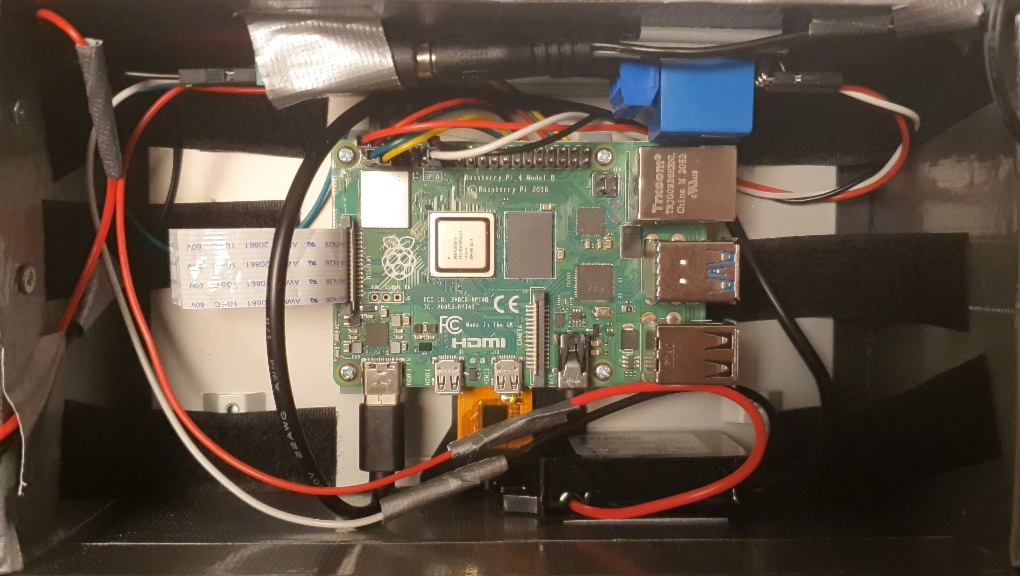
\includegraphics[width=0.9\textwidth]{images/core/schaltung.jpg}
        \caption{Die elektronische Schaltung innerhalb der Box}
    \end{center}
\end{figure}